\usetikzlibrary{matrix,chains,positioning,decorations.pathreplacing,arrows}
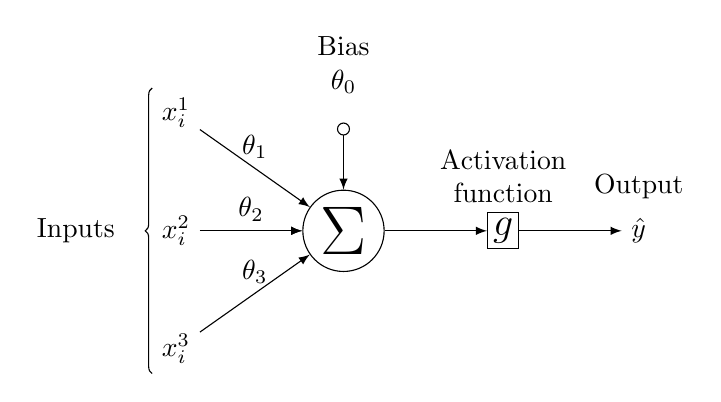
\begin{tikzpicture}[
    init/.style={
      draw,
      circle,
      inner sep=2pt,
      font=\Huge,
      join = by -latex
    },
    squa/.style={
      draw,
      inner sep=2pt,
      font=\Large,
      join = by -latex
    },
    start chain=2,node distance=13mm
    ]
    \node[on chain=2] 
      (x2) {$x_i^2$};
    \node[on chain=2,init] (sigma) 
      {$\displaystyle\Sigma$};
    \node[on chain=2,squa,label=above:{\parbox{2cm}{\centering Activation \\ function}}]   
      {$g$};
    \node[on chain=2,label=above:Output,join=by -latex] 
      {$\hat{y}$};
    \begin{scope}[start chain=1]
    \node[on chain=1] at (0,1.5cm) 
      (x1) {$x_i^1$};
    \end{scope}
    \begin{scope}[start chain=3]
    \node[on chain=3] at (0,-1.5cm) 
      (x3) {$x_i^3$};
    \end{scope}
    \node[label=above:\parbox{1.5cm}{\centering Bias \\ $\theta_0$}] at (sigma|-x1) (b) {};

    \draw[-latex] (x1) -- (sigma) node[midway,above] {$\theta_1$};
    \draw[-latex] (x2) -- (sigma) node[midway,above] {$\theta_2$};
    \draw[-latex] (x3) -- (sigma) node[midway,above] {$\theta_3$};
    \draw[o-latex] (b) -- (sigma);

    \draw[decorate,decoration={brace,mirror}] (x1.north west) -- node[left=10pt] {Inputs} (x3.south west);
\end{tikzpicture}